\chapter{Benchmarking Results}\label{chapter:analysis}

The results presented in this chapter have been calculated on a x64 architecture (Intel(R) Core(TM) i5-6200U CPU @ 2.30GHz) running Ubuntu 20.04.1 LTS. The installed docker version was 19.03.8. The benchmarking suite was initialized to run callgrind and massif 100 times, respectively (e.g. $N=100$). All values presented in this chapter are averages over $N=100$ samples. Additionally, all graphs contain the standard deviation (if no standard deviation can be observed in a particular graph, the value is zero or too small to be drawn). The exact values and the identified execution hotspots for all implementations instantiated respectively with all parameter sets (see \autoref{sec:included_implementations}) can be found in addenda \ref{app:detailed_benchmarks}. The efficiency in this chapter is quantified by the peak memory consumption and by the absolute instruction count measured by the benchmarking suite (details in \autoref{chapter:benchmarking_suite}). \\
The graphs below use the following terminology:
Assume Alice (A) and Bob (B) want to establish a shared secret using a \gls{SIDH} key exchange.
\begin{itemize}
\item \textit{KeygenA} describes the key generation (public and private key) of Alice.
\item \textit{KeygenB} describes the key generation (public and private key) of Bob.
\item \textit{SecretA} describes the computation of the shared secret by Alice.
\item \textit{SecretB} describes the computation of the shared secret by Bob.
\end{itemize}
This chapter starts with a comparison between all \gls{SIDH} security levels in \autoref{sec:analysis_sidh_levels}. This demonstrates the performance differences of the available parameter sets. \\
A comparison among all available \gls{SIKE} implementations is given in \autoref{sec:analysis_sike}: This section  works out differences between \textit{reference}, \textit{generic optimized}, \textit{x\_64 optimized} and \textit{compressed} implementations of SIKE. Moreover, the previously mentioned similarities and differences between \gls{PQCrypto-SIDH} and \gls{SIKE} are investigated based on the measured benchmarking results. \\
In \autoref{sec:sike_vs_circl} the comparison between \gls{SIKE} and \gls{CIRCL} is drawn to identify the most performant SIDH key exchange implementation. This section also analyses the observed execution hotspots of both libraries.\\
Differences in terms of efficiency between modern state-of-the-art \gls{ECDH} and quantum-resistant \gls{SIDH} are pointed out in \autoref{sec:analysis_effiency_ecdh}. This section also highlights execution hotspots measured for \gls{ECDH}. Note that all graphs in this section contain \gls{ECDH} benchmarks as reference value. However, mainly \autoref{sec:analysis_effiency_ecdh} will investigate and analyze the differences.\\
The chapter concludes with security considerations for all benchmarked implementations in terms of constant time cryptography and key size (\autoref{sec:analysis_security}).\\
At the end of each section a short summary of the results for the respective section can be found. 

\section{Comparing of \gls{SIDH} security levels}\label{sec:analysis_sidh_levels}
Before drawing any differences between libraries or implementations, this section considers the proposed parameter sets for isogeny based cryptography \parencite{sike2020spec}: \texttt{p434}, \texttt{p503}, \texttt{p610} and \texttt{p751}. Each parameter set  corresponds with a  \gls{NIST} security level (see \autoref{sidh_security} for details). This section visualizes the claimed resources of the different parameter sets for a single \gls{SIDH} key exchange. \gls{SIKE} (\autoref{sec:levels_sike}) and \gls{CIRCL} (\autoref{sec:levels_circl}) are investigated separately. Additionally, this section also compares the proposed \gls{SIDH} parameters to classical elliptic curve cryptography parameters: \texttt{secp256}, \texttt{secp384} and \texttt{secp521}. Recall the security classes of all parameter sets:

\begin{table}[H]
	\centering
	\begin{tabular}{|K{4cm}|K{4cm}|K{4cm}|}
	\hline
	\rowcolor{lightgray!50}
	\bfseries\makecell{Security Level} & \bfseries\makecell{SIDH parameters} & \bfseries\makecell{ECDH parameters} \\
	\hline
	\makecell{\gls{NIST} level 1} & \makecell{p434} & \makecell{secp256} \\
	\hline
	\makecell{\gls{NIST} level 2} & \makecell{p503} & \makecell{-} \\
	\hline
	\makecell{\gls{NIST} level 3} & \makecell{p610} & \makecell{secp384} \\
	\hline
	\makecell{\gls{NIST} level 5} & \makecell{p751} & \makecell{secp521} \\
	\hline
	\end{tabular}
	\caption[NIST security levels with SIDH and ECDH parameters]{NIST security levels with SIDH and ECDH parameters.}
	\label{tab:benchmarks_Sike_x64}
\end{table}


\subsection{Security levels of SIKE}\label{sec:levels_sike}
This section evaluates the performance of the different parameter sets implemented in the \gls{SIKE} library.  \gls{SIKE} supports all proposed parameter sets: \texttt{p434}, \texttt{p503}, \texttt{p610} and \texttt{p751}. The comparison is based on the \texttt{SIKE\_x64} implementation.\\
\autoref{fig:results_all_curves_sike} shows the absolute instruction counts for \texttt{SIKE\_x64} initialized with all available parameter sets. While \texttt{p434} executes 18 million instructions for \textit{KeygenA}, \texttt{p751} requires 67 million operations ($3.7$ times more). Roughly the same can be observed regarding \textit{KeygenB}, \textit{SecretA} and \textit{SecretB}. The other parameter sets \texttt{p503} and \texttt{p610} almost lie on a linear line between the highest and lowest security class. At the same time the \gls{ECDH} implementations are clearly faster while providing the same security levels: \texttt{Secp256} processes in total 1.7 million instructions while \texttt{p434} executes 69 million operations (40.6 times more) for a single \gls{SIDH} key exchange. \texttt{Secp384} (40 million) executes 4.3 times more instructions than \texttt{p610} (170 million) and \texttt{secp521} (96 million) executes 2.6 times more instructions than \texttt{p751} (253 million).\\
The measured peak memory consumption is for \texttt{p751} the highest ($13.3$ \gls{kB}) and for \texttt{p434} the lowest ($8.2$ \gls{kB}) among \gls{SIDH} parameters. Again, the other parameter sets can be found in between of these boundary values (\autoref{fig:results_all_curves_sike_mem}). Moreover, one can observe an increased memory consumption of \gls{ECDH} parameters: Compared to \texttt{p434}, the elliptic curve parameter set \texttt{secp256} demands 4 $kB$ more memory. \texttt{Secp384} and \texttt{secp521} allocate 3 $kB$ additionaly memory compared to their appropriate \gls{SIDH} parameters, respectively.\\\\
This analysis clearly demonstrates that an increased security level of \gls{SIDH} corresponds with a increased claim of resources. Whereas the difference in terms of memory consumption is relatively small, the execution times differ noticably: On average and compared to \texttt{p434} the parameter set
\begin{itemize}
\itemsep0em 
\item \texttt{p503} executes $1.4$ times more instructions
\item \texttt{p610} executes $2.5$ times more instructions
\item \texttt{p710} executes $3.7$ times more instructions
\end{itemize}
While the \gls{ECDH} parameter sets enable faster computation times for a single key exchange, they also suffer from an increased memory consumption. The reason for this might be a trade-off between execution time and memory consumption (e.g. \parencite{1056220}). An analysis of this trade-off, however, requires further investigation beyond the scope of this work.
\begin{figure}[H]
  \centering
  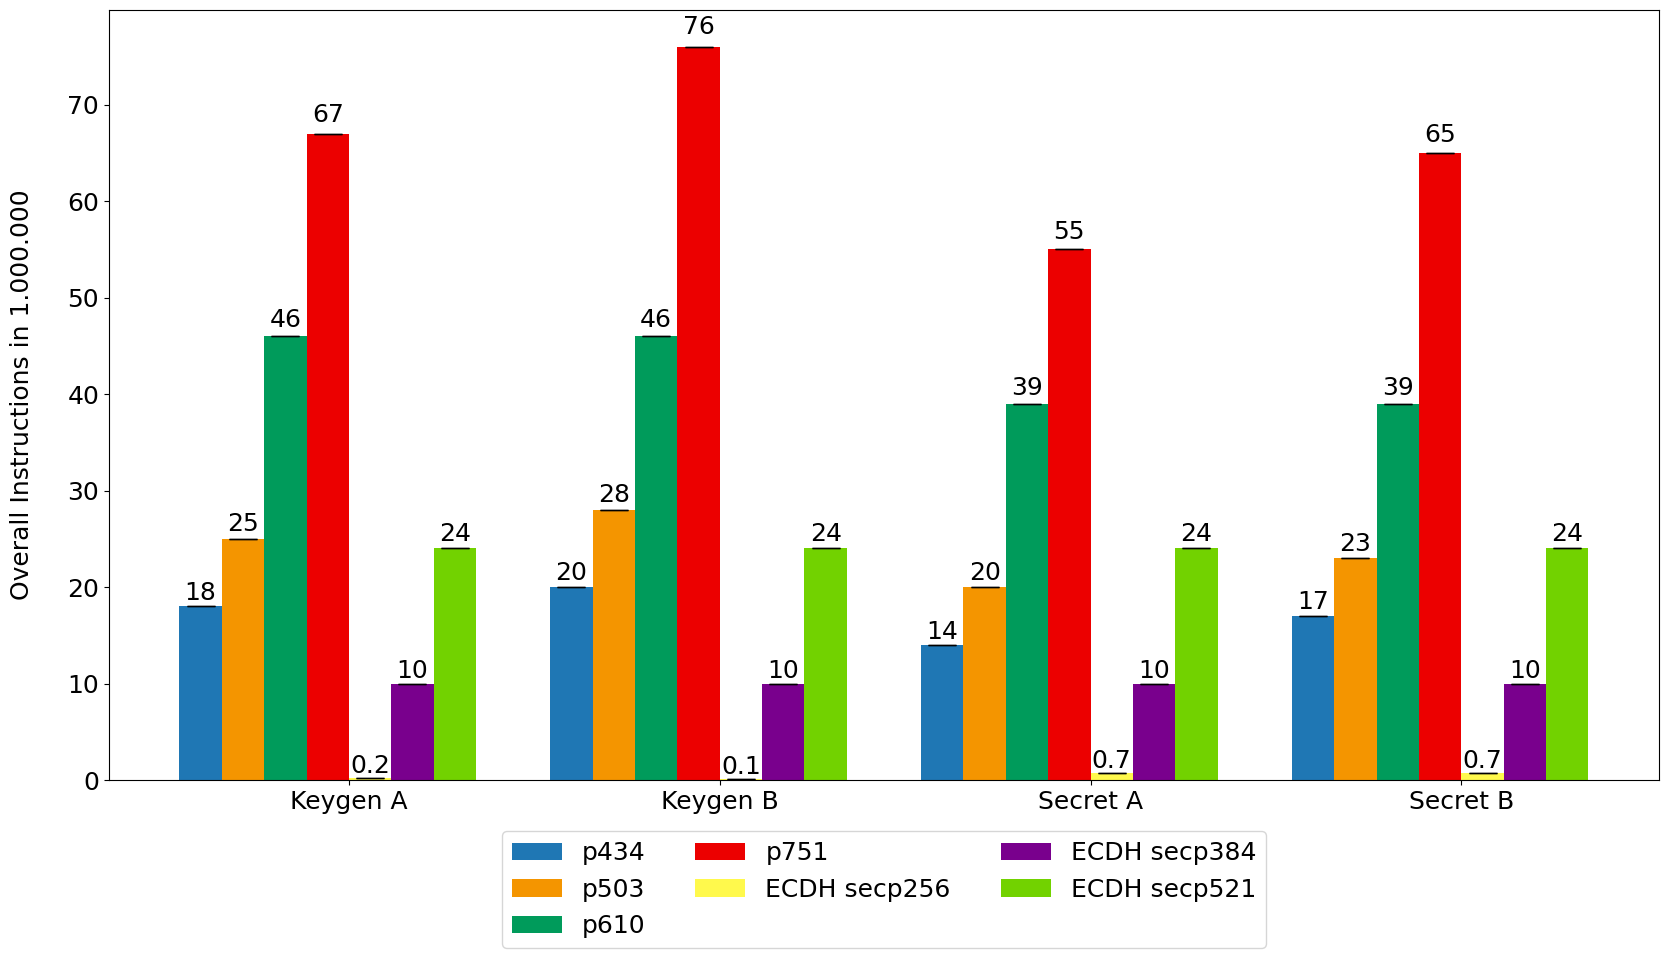
\includegraphics[width=0.9\textwidth]{benchmarks/compare_sidh_parameters/sike/Sike_x64}
  \caption[Overall instructions for all parameter sets via \texttt{SIKE\_x64} compared to \texttt{ECDH}]
  {Overall instructions for \texttt{SIKE\_x64} initiated with all possible parameter sets compared to appropriate \texttt{ECDH} parameter sets.}
  \label{fig:results_all_curves_sike}
\end{figure}

\begin{figure}[H]
  \centering
  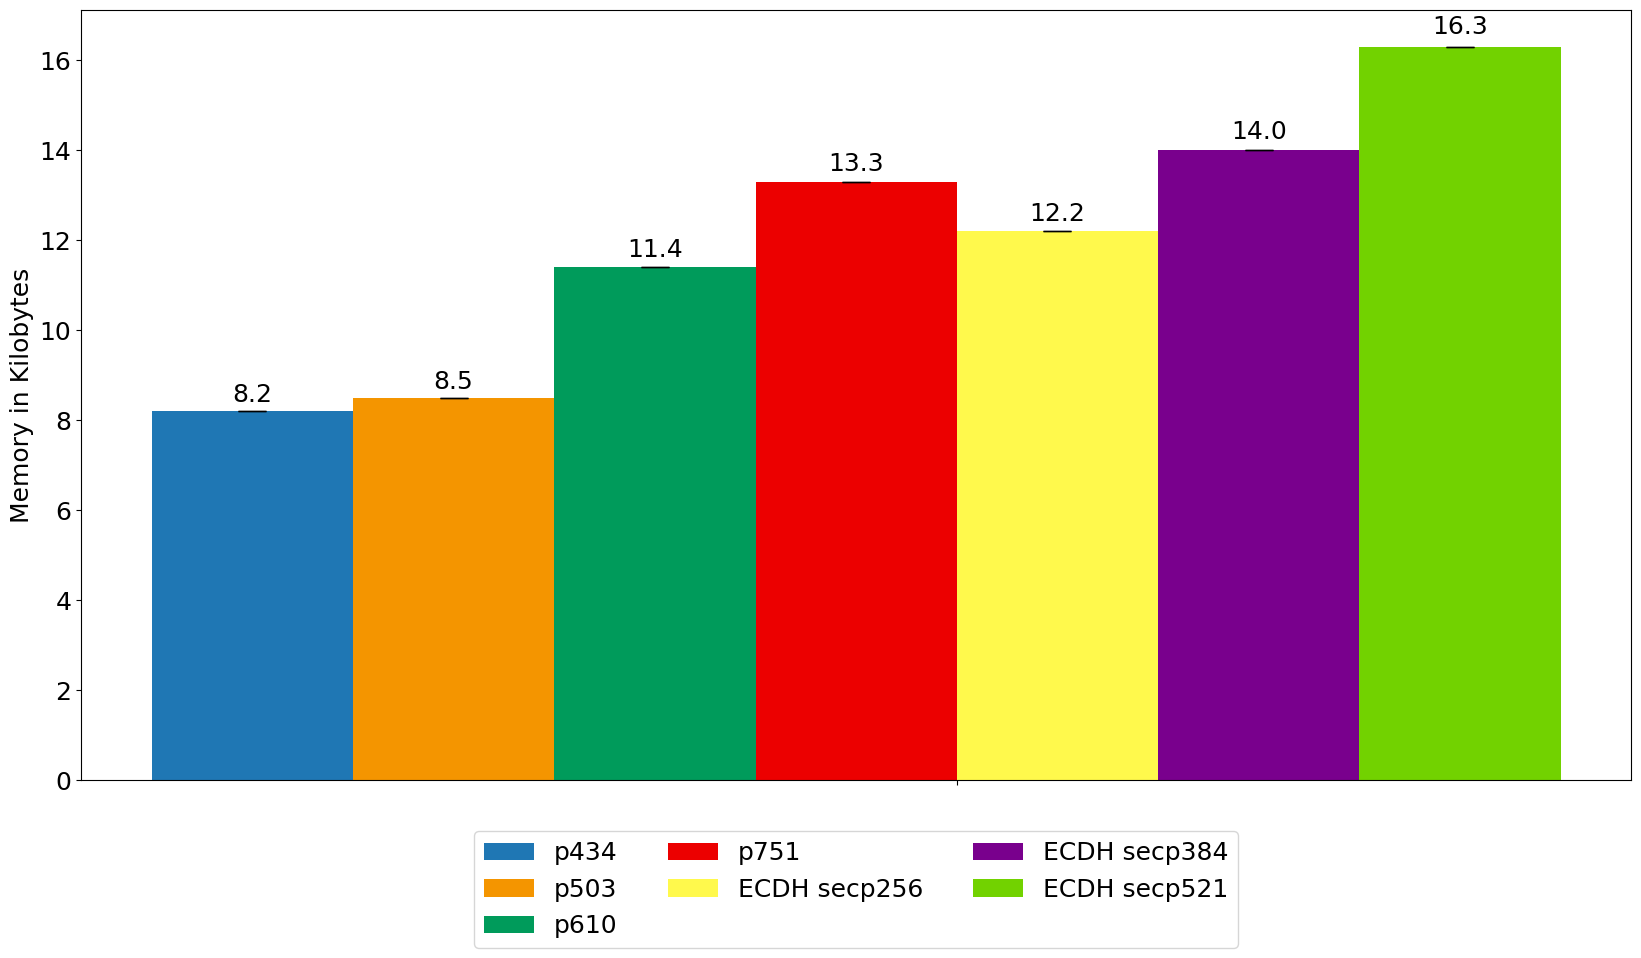
\includegraphics[width=0.9\textwidth]{benchmarks/compare_sidh_parameters/sike/Sike_x64_mem}
  \caption[Maximum memory consumption for all parameter sets via \texttt{SIKE\_x64}  compared to \texttt{ECDH}]
  {Maximum memory consumption in kilobytes of \texttt{SIKE\_x64} initiated with all possible parameter sets compared to appropriate \texttt{ECDH} parameter sets.}
  \label{fig:results_all_curves_sike_mem}
\end{figure}

\subsection{Security levels of CIRCL}\label{sec:levels_circl}
This section evaluates the performance of the different parameter sets implemented in the \gls{CIRCL} library. \gls{CIRCL} supports the following parameter sets: \texttt{p434}, \texttt{p503}, and \texttt{p751}. The comparison is based on the \texttt{CIRCL\_x64} implementation.\\\\
\autoref{fig:results_all_curves_circl} visualizes the executed instructions of all implemented parameter sets in \gls{CIRCL}. Additionally, the graph also shows the benchmarks for ECDH and the appropriate parameters (\texttt{p434} matching \texttt{secp256} and \texttt{p751} matching \texttt{secp521}). As expected, \texttt{p434} is the fastest implementation among the \gls{SIDH} parameter set (this holds for all categories). In total a whole key exchange using parameter \texttt{p434} processes 101 million instructions, while parameter \texttt{p503} (114 million) is slightly slower and parameter \texttt{p751} (359 million) is by far the slowest version. The overhead of processed instructions for \texttt{p751} compared to the other parameter sets is significant.
When comparing \gls{CIRCL} to \gls{ECDH} a significant speed difference can be observed: \texttt{Secp256} executes in total 1.7 million instructions (95 times less than \texttt{p434}) and texttt{Secp521} executes in total 96 million instructions (4 times less than \texttt{p751}). Thus, \gls{ECDH} is clearly faster for both parameter sets.\\
The analysis of the allocated memory of the different parameter sets reveals a dynamic allocation behavior of the \gls{CIRCL} library (\autoref{fig:results_all_curves_circl_mem}). For each parameter set the peak memory consumption varies between multiple measurements (see the standard deviation in the graph). The claimed memory for the different parameter sets is almost equal: \texttt{p434} allocates on average about 22 \gls{kB} memory, \texttt{p503} about 21.6 \gls{kB} and \texttt{p751} about 23.1 \gls{kB}. At the same time \gls{CIRCL} allocates more memory than \gls{ECDH}: \texttt{Secp256} uses 12.2 \gls{kB} memory  and \texttt{Secp521} allocates 16.3 \gls{kB}.\\

Increased security levels of \gls{SIDH} corresponds with a increased amount of executed instructions. Compared to \texttt{p434} the parameter set
\begin{itemize}
\itemsep0em 
\item \texttt{p503} executes on average $1.1$ times more instructions
\item \texttt{p710} executes on average $3.6$ times more instructions
\end{itemize}

The observed dynamic memory allocation behavior of \gls{CIRCL} might be a consequence of the garbage collector implemented in the Go language \parencite{Hudson:GGC}. The GO garbage collector starts in parallel with the main executable on multi processor architectures \parencite{go2020faq}. Due to the state of the CPU during execution and dynamic cache behavior garbage collection could free memory in a non-deterministic process. This might lead to a different peak memory consumption during multiple runs of the binary. \\
The observed memory allocations by \gls{CIRCL} marginally differ for different parameter sets. Again, an explanation for this behavior could be the GO garbage collector. The garbage collector knows an upper bound of memory that might be allocated by a binary. Once this upper bound is reached the garbage collector gets active and frees unused memory \parencite{Hudson:GGC}.

\begin{figure}[H]
  \centering
  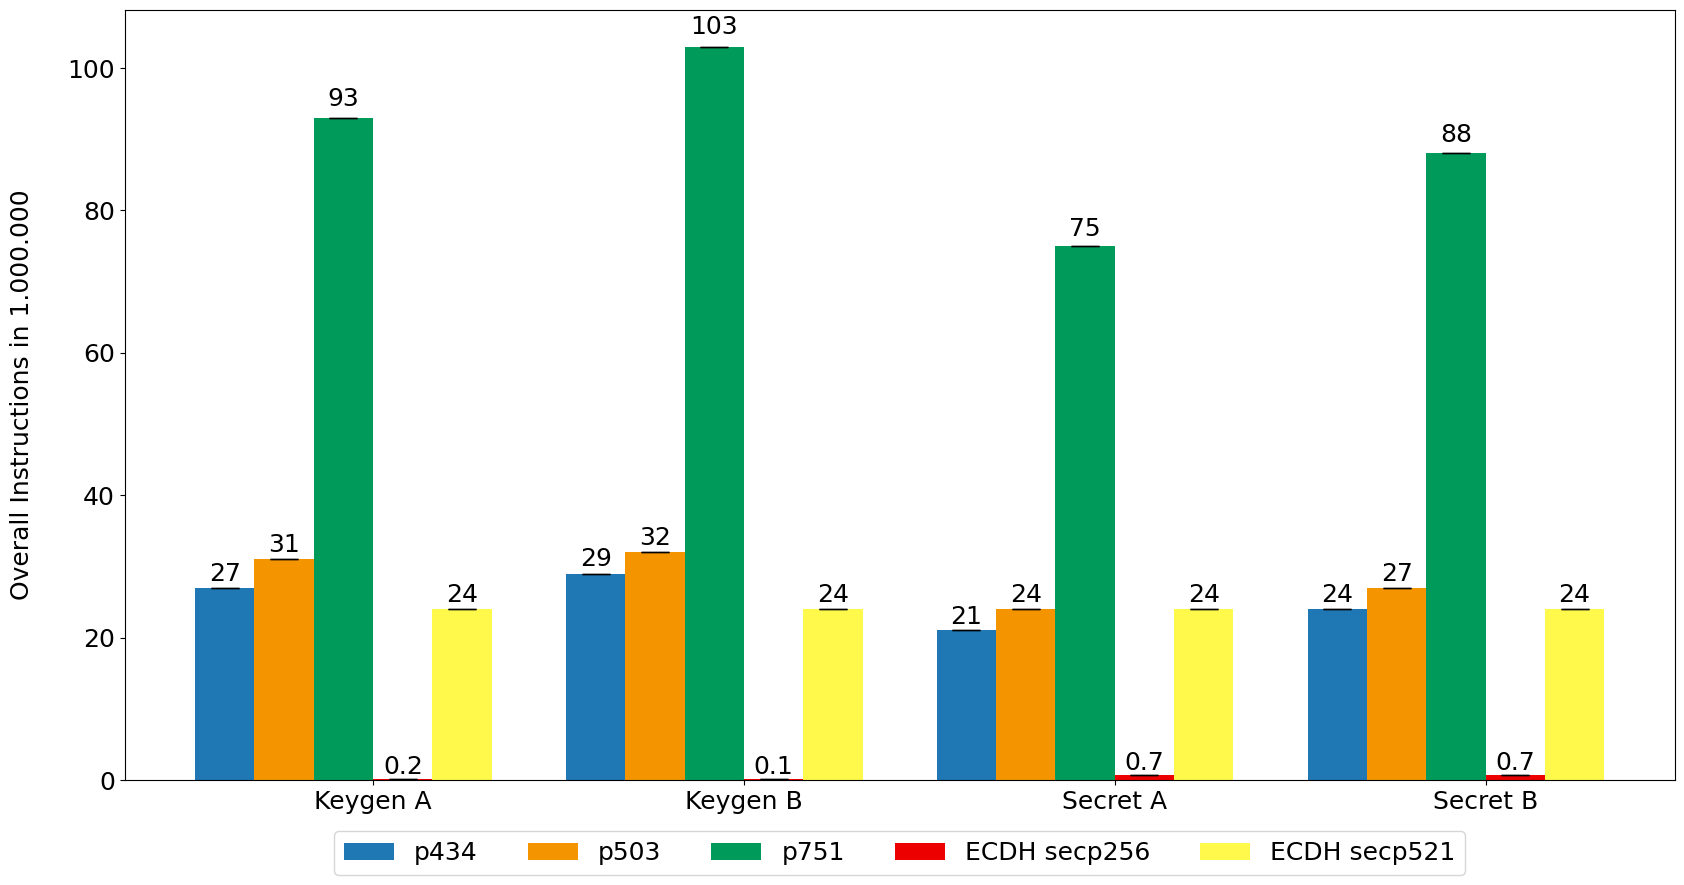
\includegraphics[width=0.9\textwidth]{benchmarks/compare_sidh_parameters/circl/CIRCL_x64}
  \caption[Overall instructions for all parameter sets via \texttt{CIRCL\_x64} compared to \texttt{ECDH}]
  {Overall instructions for \texttt{CIRCL\_x64} initiated with all possible parameter sets compared to appropriate \texttt{ECDH} parameter sets.}
  \label{fig:results_all_curves_circl}
\end{figure}

\begin{figure}[H]
  \centering
  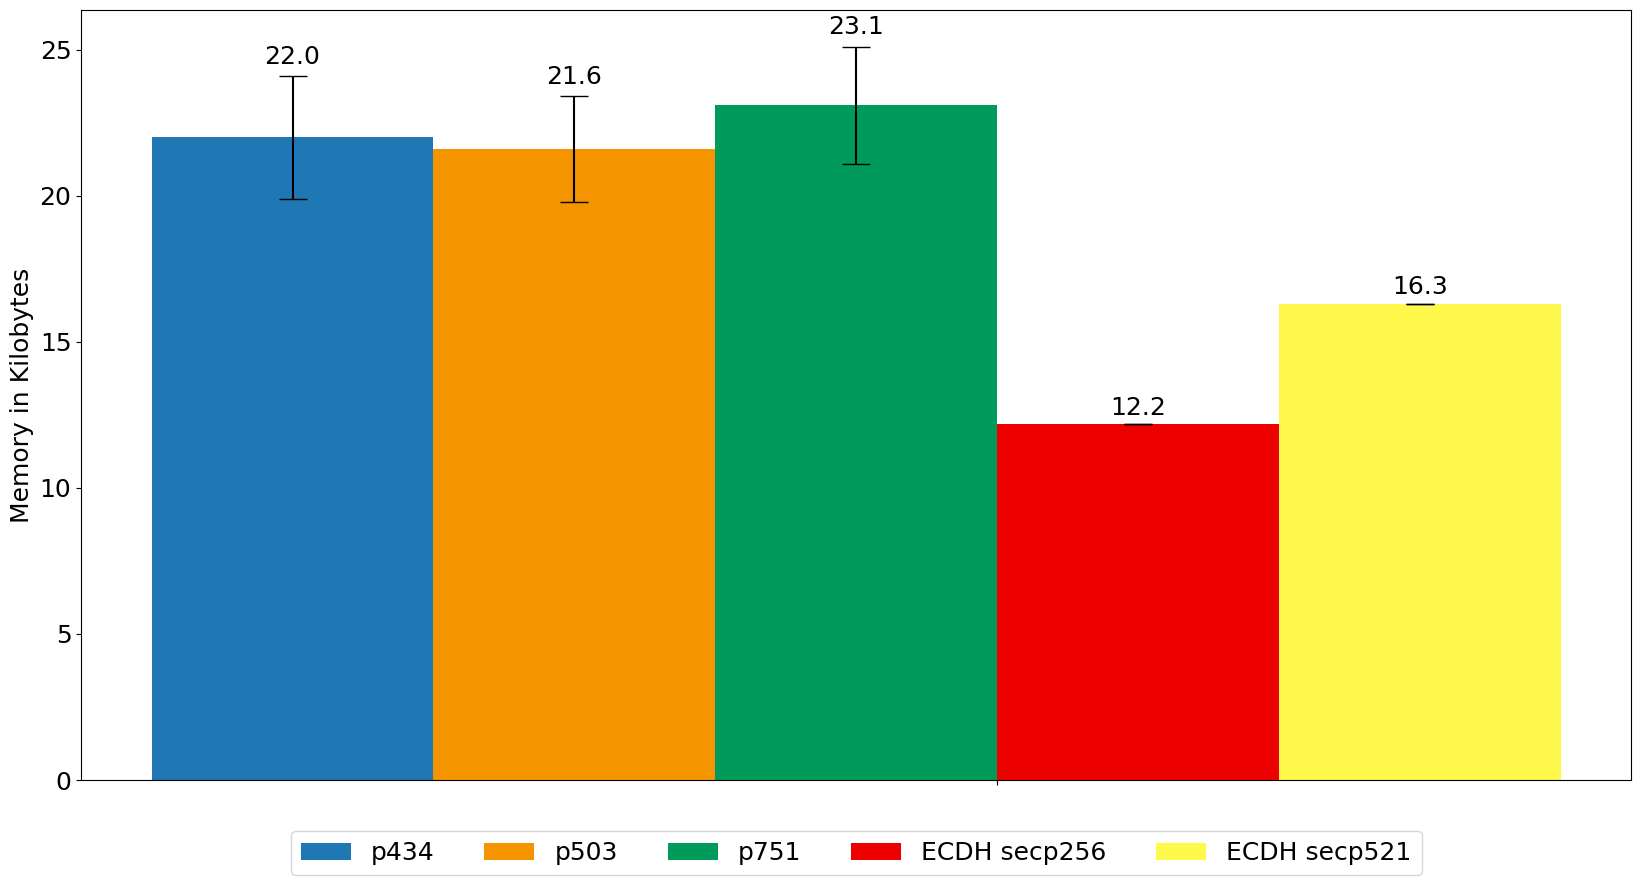
\includegraphics[width=0.9\textwidth]{benchmarks/compare_sidh_parameters/circl/CIRCL_x64_mem}
  \caption[Maximum memory consumption for all parameter sets via \texttt{CIRCL\_x64}  compared to \texttt{ECDH}]
  {Maximum memory consumption in kilobytes of \texttt{CIRCL\_x64} initiated with all possible parameter sets compared to appropriate \texttt{ECDH} parameter sets.}
  \label{fig:results_all_curves_circl_mem}
\end{figure}

\subsection{Summary of findings}
This section reveals that an increased level of security does not necessarily correspond with an linear increase of resources. While this assumption holds for the \gls{SIKE} library, the GO runtime (e.g. the GO garbage collector) affects the benchmarks for the \gls{CIRCL} library. Thus, the chosen programming language influences the claimed resources of \gls{SIDH} security parameters.\\
\gls{ECDH} is faster for all security parameters than \gls{SIKE} and \gls{CIRCL}. However, \gls{SIKE} requires less memory than \gls{ECDH} (might be caused by a time-space trade-off).

\section{Comparing \gls{SIKE} implementations}\label{sec:analysis_sike}
Before the comparisons between the \gls{SIDH} libraries \textit{\gls{SIKE}} and \textit{\gls{CIRCL}} are drawn, the differences of available \textit{\gls{SIKE}} implementations are investigated. Besides a \textit{reference} implementation, the library provides \textit{generic optimized} and \textit{x64 optimized} variants. This section analyzes the differences between these \textit{optimized} implementations. Moreover,  \textit{compressed} versions for both \textit{optimized} variants are available. The performance differences between \textit{compressed} and \textit{non-compressed} versions are additionally emphasized in this section. Since the previous section investigated differences between \gls{SIDH} parameter sets this section only considers \texttt{p434}. The analysis of detailed benchmarks listed in addenda \ref{app:detailed_benchmarks} for other parameter sets (\texttt{p503}, \texttt{p610} and \texttt{p751}) lead to similar results as presented in this section.


\subsubsection{Reference implementation}
The \texttt{SIKE\_Reference} implementation is with 11.2 \gls{kB} allocated memory close to the average ($\sim$ 12.7 \gls{kB}) of all \gls{SIKE} implementations (see \autoref{fig:results_sike_mem}). Regarding the execution times for key generation in \autoref{fig:results_sike}, the reference implementation is by far the slowest variant: More than 2.3 billion ($2.300.000.000$) instructions were measured in order to generate Bobs key pair. This is slower by factor 100 compared to \texttt{SIKE\_x64}. As the name suggests, this reference implementation must be seen as a proof-of-concept. Thus, performance criteria are no requirements for this implementation, which is confirmed by the observed benchmarking results.

\subsubsection{Optimized implementations}
\gls{SIKE} provides two \textit{optimized} implementations: \texttt{SIKE\_Generic} and \texttt{SIKE\_x64}. \texttt{SIKE\_x64} is optimized for the x64 instruction set taking advantage of architecture specific operations. \texttt{SIKE\_Generic} implements generic code without optimizing code for a concrete architecture. Both variants are clearly faster than the reference implementation meeting intuitive expectations. The benchmarks in \autoref{fig:results_sike} show a significant speed up of \texttt{SIKE\_x64} compared to \texttt{SIKE\_Generic}. Key generation for Alice and Bob is 10.8 times faster and secret generation about 11 times. At the same time \texttt{SIKE\_Generic} allocates 7.7 \gls{kB} memory, which is 0.5 \gls{kB} less than the x64 optimized variant (\autoref{fig:results_sike_mem}). Thus, the increased speed involves the allocation of more memory -- a time-memory trade-off (e.g. \parencite{1056220}). At the same time these benchmarks show the advantage of optimizing \gls{SIDH} for a concrete hardware architecture instead of providing a generic implementation.

\subsubsection{Compressed implementations}
\gls{SIKE} provides compressed variants for both optimized implementations:\\ \texttt{SIKE\_Generic\_Compressed} and \texttt{SIKE\_x64\_Compressed}.
Both \textit{compressed} versions also contain \textit{optimized} code. Their key sizes, however, are reduced compared to non-compressed variants. In order to reduce the key sizes these algorithms implement functions to compress and to decompress cryptographic keys.\\
\autoref{fig:results_sike} clearly shows a difference between \textit{optimized} and \textit{compressed} versions of \gls{SIKE} in terms of absolute instructions. Compressed versions roughly claim twice as much operations ($\sim$ 500 million for \texttt{SIKE\_Generic\_Compressed} and $\sim$ 45 million \texttt{SIKE\_x64\_Compressed}) to generate a key pair as non-compressed variants ($\sim$ 200 million for \texttt{SIKE\_Generic} and $\sim$ 19 million \texttt{SIKE\_x64}). Additionally, the generation of the shared secret using \textit{compressed} implementations is slightly slower. For all \textit{compressed} versions the executed instructions vary (see the standard deviation) because the compression of the public keys depend on the generated key, which is different for each \gls{SIDH} key exchange.\\
Besides execution times, \autoref{fig:results_sike_mem} also compares the memory consumption. As stated by the authors of \gls{SIKE}, compressed variants allocate more memory~\parencite{sike2020spec}: The peak memory allocation is with 17 kilobytes (\texttt{SIKE\_Generic\_Compressed}) and 19.2 kilobytes (\texttt{SIKE\_x64\_Compressed}) twice as high as for the non-compressed versions. The measured peak memory consumption is constant for \textit{compressed} implementations and does not vary.\\
This shows that \textit{optimized} versions have reduced execution times as well as decreased memory consumption compared to \textit{compressed} implementations. Roughly speaking, \textit{compressed} versions demand twice as much resources than \textit{optimized} variants, while decreasing the effective key sizes (see \autoref{sec:analysis_security_keys} for details). Since the compression and decompression force additional steps during a \gls{SIDH} key exchange these variants the increased claim of resources is reasonable.



\begin{figure}[H]
  \centering
  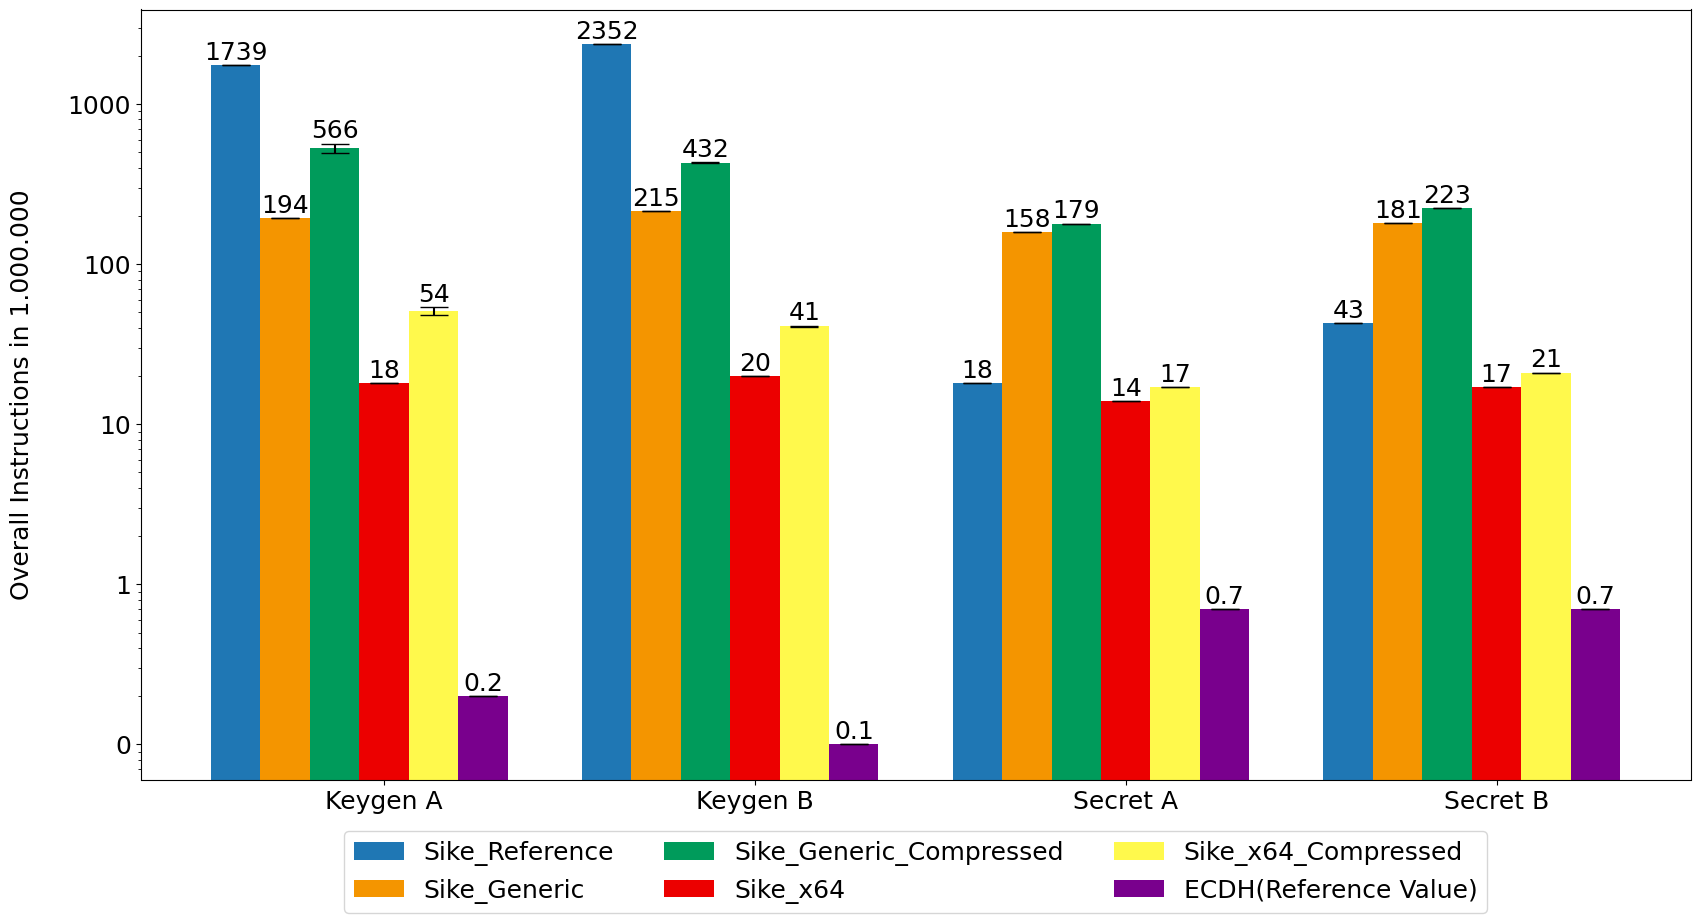
\includegraphics[width=1\textwidth]{benchmarks/compare_sike/compressed/sike}
  \caption[Overall instructions \gls{SIKE}]
  {Overall instructions for all \gls{SIKE} implementations initialized with \texttt{p434}. \gls{ECDH} is shown as reference value using parameter \texttt{secp256}.}
  \label{fig:results_sike}
\end{figure}

\begin{figure}[H]
  \centering
  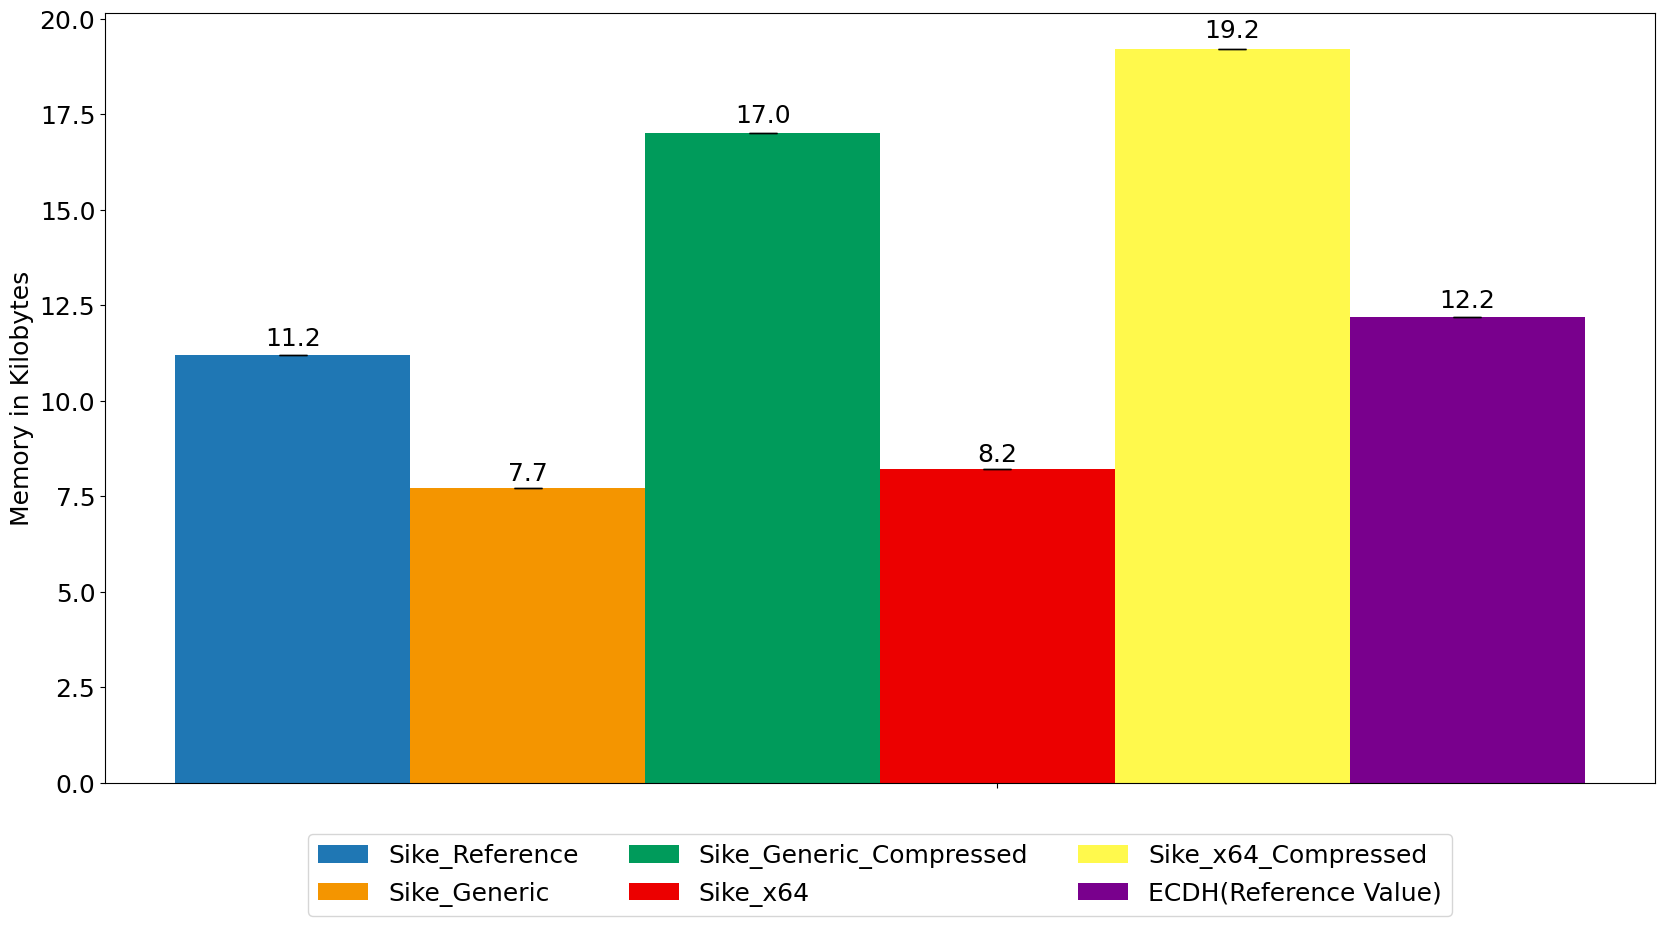
\includegraphics[width=1\textwidth]{benchmarks/compare_sike/compressed/sike_mem}
  \caption[Maximum memory consumption \gls{SIKE}]
  {Maximum memory consumption in kilobytes or all \gls{SIKE} implementations initialized with \texttt{p434}. \gls{ECDH} is shown as reference value using parameter \texttt{secp256}.}
  \label{fig:results_sike_mem}
\end{figure}

\subsection{\gls{PQCrypto-SIDH} vs. \gls{SIKE}}

This section describes the similarities and differences between \gls{PQCrypto-SIDH} and \gls{SIKE}. Note, that the \gls{SIKE} team uses the Microsoft Github repository of \gls{PQCrypto-SIDH} to create their \gls{NIST} submissions (see \autoref{existing:sike_vs_pqcrypto} for details). This similarity can be observed when analyzing the \textit{optimized} implementations. At the same time the benchmarked versions of the libraries reveal considerable differences when analyzing their \textit{compressed} versions. This is investigated in the following sections.

\subsubsection{Optimized implementations}
This section compares the \textit{optimized} implementations of \gls{SIKE} and \gls{PQCrypto-SIDH}: \texttt{SIKE\_Generic}, \texttt{SIKE\_x64}, \texttt{Microsoft\_Generic} and  \texttt{Microsoft\_x64}.
Generic optimized implementations contain generally optimized code for various hardware platforms. In contrast, x64 optimized variants exploit hardware specific instructions. 

\autoref{fig:results_sike_pqc_opt_434} shows the benchmarks for execution time of the optimized variants initiated with \texttt{p434}. In all four steps of the \gls{SIDH} key exchange, the benchmarked values for both libraries look almost the same. However, when considering exact measurements from  \ref{app:detailed_benchmarks}, one can observe that \textit{SIKE\_Generic} executes constantly half a million operations less than \textit{Microsoft\_Generic} (this holds for all four categories: Keygen A, Keygen B, Secret A and Secret B). While this sounds significant, the relative difference is actually less than $0.01$\%. While the absolute gap further increases, when higher security classes are analyzed (about three million operations constant difference for \texttt{p751}), the relative disparity stays below $0.01$\%. Similar results can be observed for \textit{SIKE\_x64} and \textit{Microsoft\_x64}. There are almost no differences between the two libraries for \textit{optimized} implementations considering the counted instructions.
\\\\
Peak memory consumptions for parameter \textit{p434} are visualized in  \autoref{fig:results_sike_pqc_opt_434_mem}. As in terms of execution time, memory allocation numbers between \textit{SIKE\_Generic} and \textit{Microsoft\_Generic} marginally differ: The \gls{SIKE} version occupies $0.3$ \gls{kB} less memory for \textit{p434} and $0.6$ \gls{kB} less than for \textit{p751}. Overall, the relative difference regarding memory consumption is about $5$\%. Again, the same is valid for \textit{SIKE\_x64} and \textit{Microsoft\_x64}: The Microsoft implementation allocates $0.7$ \gls{kB} more memory for \textit{p434} and $1.7$ \gls{kB} more than for \textit{p751}.
\\\\
Both implementations hardly differ in their performance benchmarks. This analysis reveals the similarities of the libraries \gls{SIKE} and \gls{PQCrypto-SIDH}. The fact that both libraries relay on the same software stack is mirrored in the benchmark results. The slight performance differences are might be caused by the different software releases used for benchmarking.

\begin{figure}[H]
  \centering
  \includegraphics[width=1\textwidth]{benchmarks/compare_sike/compare_pqc_sike/optimized/434}
  \caption[Overall instructions for optimized implementations of \gls{SIKE} and \gls{PQCrypto-SIDH} using \texttt{p434}]
  {Overall instructions for optimized implementations of \gls{SIKE} and \gls{PQCrypto-SIDH} using \texttt{p434} compared to \gls{ECDH} via \texttt{secp256r1}.}
  \label{fig:results_sike_pqc_opt_434}
\end{figure}

\begin{figure}[H]
  \centering
  \includegraphics[width=1\textwidth]{benchmarks/compare_sike/compare_pqc_sike/optimized/434_mem}
  \caption[Maximum memory consumption for optimized implementations of \gls{SIKE} and \gls{PQCrypto-SIDH} using \texttt{p434}]
  {Maximum memory consumption in kilobytes for optimized implementations of \gls{SIKE} and \gls{PQCrypto-SIDH} using \texttt{p434} compared to \gls{ECDH} via \texttt{secp256r1}.}
  \label{fig:results_sike_pqc_opt_434_mem}
\end{figure}

\subsubsection{Compressed implementations}
Recall that compressed implementations of \gls{SIDH} promise shortened key size compared to non-compressed versions, however, this leads to increased execution times and memory allocations. As mentioned above the benchmarked \gls{SIKE} version (Round 2 submission) does not implement the latest optimizations for compressed versions. However, the analyzed version of \gls{PQCrypto-SIDH} already integrates these improvements. Thus, this section reveals the differences between the benchmarked versions of \gls{SIKE} and \gls{PQCrypto-SIDH}, which is in particular the integration of faster compressing algorithms \parencite{cryptoeprint:2020:431}.\\
\autoref{fig:results_sike_pqc_comp_434} shows the execution time benchmarks for the compressed variants of \gls{PQCrypto-SIDH} and \gls{SIKE} initiated with \texttt{p434}. Naturally, the x64 optimized code is faster than the generic optimization. The Microsoft implementations executed less operations than \gls{SIKE}: Regarding key generation, \textit{SIKE\_Generic\_Compressed} performed on average $38$\% more instructions than \textit{Microsoft\_Generic\_Compressed}. \textit{SIKE\_x64\_Compressed} performed on average $45$\% more instructions than \textit{Microsoft\_x64\_Compressed}. The generation of the secret key only shows slight differences between \gls{SIKE} and Microsoft, however Microsoft remains the fastest. The trend of this analysis also applies to improved security classes, e.g to parameter \textit{p751} (see \autoref{fig:results_sike_pqc_comp_751}). Again, these compressed algorithms vary in terms of executed instructions (see the standard deviation), since the effort for compressing a key depend on the key itself. Since the keys are generated at runtime no static amount of instructions can be observed.
\\
The following evaluation of the allocated memory is surprising (\autoref{fig:results_sike_pqc_comp_434_mem}): The Microsoft implementations occupy three times more memory than \gls{SIKE} when initiated with \textit{p434}. This gap rises strongly when increasing the security class to \textit{p751} (\autoref{fig:results_sike_pqc_comp_751_mem}), where the \textit{ \gls{PQCrypto-SIDH}} library of Microsoft allocates almost seven times more memory.
\\\\
While the benchmarks for the compressed Microsoft implementations reveal faster execution times, the overhead of allocated memory compared to \gls{SIKE} is enormous. The observed differences are the results of the integration of optimized compression algorithms \parencite{cryptoeprint:2020:431}: Reducing the execution times for compression directly increases the memory consumption of the algorithms -- a time-memory trade-off.


\begin{figure}[H]
  \centering
  \includegraphics[width=1\textwidth]{benchmarks/compare_sike/compare_pqc_sike/compressed/434}
  \caption[Overall instructions for compressed implementations of \gls{SIKE} and \gls{PQCrypto-SIDH} using \texttt{p434}]
  {Overall instructions for compressed implementations of \gls{SIKE} and \gls{PQCrypto-SIDH} using \texttt{p434} compared to \gls{ECDH} via \texttt{secp256r1}.}
  \label{fig:results_sike_pqc_comp_434}
\end{figure}

\begin{figure}[H]
  \centering
  \includegraphics[width=1\textwidth]{benchmarks/compare_sike/compare_pqc_sike/compressed/434_mem}
  \caption[Maximum memory consumption in kilobytes for compressed implementations of \gls{SIKE} and \gls{PQCrypto-SIDH} using \texttt{p434}]
  {Maximum memory consumption in kilobytes for compressed implementations of \gls{SIKE} and \gls{PQCrypto-SIDH} using \texttt{p434} compared to \gls{ECDH} via \texttt{secp256r1}.}
  \label{fig:results_sike_pqc_comp_434_mem}
\end{figure}

\begin{figure}[H]
  \centering
  \includegraphics[width=1\textwidth]{benchmarks/compare_sike/compare_pqc_sike/compressed/751}
  \caption[Overall instructions for compressed implementations of \gls{SIKE} and \gls{PQCrypto-SIDH} using \texttt{p751}]
  {Overall instructions for compressed implementations of \gls{SIKE} and \gls{PQCrypto-SIDH} using \texttt{p751} compared to \gls{ECDH} via \texttt{secp521r1}.}
  \label{fig:results_sike_pqc_comp_751}
\end{figure}

\begin{figure}[H]
  \centering
  \includegraphics[width=1\textwidth]{benchmarks/compare_sike/compare_pqc_sike/compressed/751_mem}
  \caption[Maximum memory consumption in kilobytes for compressed implementations of \gls{SIKE} and \gls{PQCrypto-SIDH} using \texttt{p751}]
  {Maximum memory consumption in kilobytes for compressed implementations of \gls{SIKE} and \gls{PQCrypto-SIDH} using \texttt{p751} compared to \gls{ECDH} via \texttt{secp521r1}.}
  \label{fig:results_sike_pqc_comp_751_mem}
\end{figure}

\subsection{Summary of findings}
The comparison among \gls{SIKE} implementations reveals significant the performance differences: The x64 optimized version (\texttt{SIKE\_x64}) is faster than the generic optimized variant (\texttt{SIKE\_Generic}). The reference implementation (\texttt{SIKE\_Reference}) is by far the slowest implementation. This is reasonable, since the reference implementation does not focus on performance. While \texttt{SIKE\_Generic} implements code for arbitrary target architectures, \texttt{SIKE\_x64} implements hardware specific instructions leading to faster execution.  Moreover, compressed versions reduce the performance for \gls{SIDH} key exchanges: In order to decrease cryptographic keys these implementations implement compression and decompression algorithms. These key transformations lead to an increased amount of executed instructions. Additionally, more memory is allocated during key (de)compression.\\
The evaluation between \gls{PQCrypto-SIDH} and \gls{SIKE} exemplarily shows, how further research might influence isogeny based cryptography. Improved compression algorithms reduced the executed instructions while the memory costs increased (space-time trade-off). At the same time, the analysis of optimized algorithms reveals the similarities between both libraries.


\section{Comparing \gls{SIKE} and \gls{CIRCL}} \label{sec:sike_vs_circl}

This section compares the SIDH libraries \gls{SIKE} and \gls{CIRCL}. Since \gls{CIRCL} does not provide any compressed versions, the analysis in this section includes the following implementations: \texttt{SIKE\_Generic}, \texttt{SIKE\_x64}, \texttt{CIRCL\_Generic} and \texttt{CIRCL\_x64}.\\
Firstly, the generic optimized implementations are compared in terms of executed instructions and allocated memory (\autoref{sec:sike_circl_analysis_generic}). Secondly, \autoref{sec:sike_circl_analysis_x64} compares the x64 optimized variants of both libraries. Finally, this chapter evaluates the measured execution hotspots for \gls{SIKE} and \gls{CIRCL} in (\autoref{sec:analysis_sidh_hotspots}). 

\subsection{Generic optimized implementations}\label{sec:sike_circl_analysis_generic}
Generic optimized implementations do not make use of any assembler specific instruction. They implement the \gls{SIDH} key exchange without any hardware assumptions resulting in  algorithms that can be executed on multiple target architectures. This section compares \texttt{SIKE\_Generic} and \texttt{CIRCL\_Generic}.\\
\autoref{fig:results_opt_434} contains the benchmarks for \gls{SIDH} key exchanges using generic implementations instantiated with \texttt{p434}.  In all four aspect of the key exchange \texttt{SIKE\_Generic} processes twice as many instructions as \texttt{CIRCL\_Generic} (factor 2). This difference even grows when considering parameter set \texttt{p751} in \autoref{fig:results_opt_751}, where \texttt{SIKE\_Generic} executes on average 2.3 times more instructions than \texttt{CIRCL\_Generic}.\\
At the same time \texttt{CIRCL\_Generic} allocates more memory than \texttt{SIKE\_Generic}: Running the benchmarks with parameter \texttt{p434} reveals a memory overhead by factor 3.1 (\autoref{fig:results_opt_434_mem}). Using parameter \texttt{p751} reduces this overhead to factor 1.9 (\autoref{fig:results_opt_751_mem}), however, this difference is still significant. Additionally, note the standard deviation for the allocated memory measured for \texttt{CIRCL\_Generic} in both graphs. The generic optimized \gls{CIRCL} implementation does not provide a constant memory consumption.
\\\\
This analysis shows, that the faster generic optimized implementation is \texttt{CIRCL\_Generic}. At the same time \texttt{SIKE\_Generic} occupies less memory -- again a trade-off between executed instructions and allocated memory can be observed (e.g. \parencite{1056220}). The benchmarked deviation of peak memory consumption by \gls{CIRCL} might be the result of the GO garbage collector\parencite{Hudson:GGC}.

\subsection{X64 optimized implementations}
\label{sec:sike_circl_analysis_x64}
X64 optimized implementations exploit specific hardware operations to improve performance for machines implementing the x64 instruction set. This section compares \texttt{SIKE\_x64} and \texttt{CIRCL\_x64}.\\
\autoref{fig:results_opt_434} shows the execution time benchmarks for all optimized variants initiated with \texttt{p434}. In all four categories listed in the graph \textit{SIKE\_x64}  is the fastest x64 implementation. \textit{CIRCL\_x64} is slower: For key generation \gls{CIRCL} processes 9 million instructions more and for generating a shared secret the library generates 7 million additional instruction compared to \gls{SIKE}. This corresponds to a relative difference of factor 1.5.
\autoref{fig:results_opt_751} compares the implementations initiated with \textit{p751} - matching the highest \gls{NIST} security level 5. \textit{SIKE\_x64} stays the faster version while the relative difference to \textit{CIRCL\_x64} (factor 1.36) decreases.
\\
In order to compare the memory consumption of the x64 optimized implementations, consider \autoref{fig:results_opt_434_mem}. The memory benchmarks of \textit{SIKE\_x64} ($8.2$ \gls{kB}) are  lower than the measured allocations of \textit{\gls{CIRCL}\_x64}, revealing  a peak allocation of $22.0$ \gls{kB} for a single \gls{SIDH} key exchange. This is by factor 2.7 greater compared to \gls{SIKE}. However, \autoref{fig:results_opt_751_mem} reveals that the memory consumption for \textit{\gls{CIRCL}\_x64} does barely change for higher security classes. Nevertheless,  \textit{\gls{CIRCL}\_x64} has a more intense memory consumption than \textit{SIKE\_x64} using \texttt{p751} (by factor 1.7). Moreover, the measured peak memory consumption of \gls{CIRCL} is not constant: Both graphs (\ref{fig:results_opt_434_mem} and \ref{fig:results_opt_751_mem}) show a considerable standard deviation during 100 runs of the x64 optimized algorithm.
\\\\
The fastest x64 optimized \gls{SIDH} key exchange is performed by \textit{SIKE\_x64}. \textit{CIRCL\_x64} is slower and allocates clearly more memory. Additionally the \gls{CIRCL} library does not implement constant memory allocations. This dynamic behavior of the binary could be a result of the garbage collector used by the GO programming language \parencite{Hudson:GGC}.

\begin{figure}[H]
  \centering
  \includegraphics[width=1\textwidth]{benchmarks/compare_circl_sike/434}
  \caption[Overall instructions of SIKE and CIRCL using \texttt{p434}]
  {Overall instructions for \gls{SIDH} parameter \texttt{p434} compared to \gls{ECDH} via \texttt{secp256r1}.}
  \label{fig:results_opt_434}
\end{figure}

\begin{figure}[H]
  \centering
  \includegraphics[width=1\textwidth]{benchmarks/compare_circl_sike/434_mem}
  \caption[Maximum memory consumption of SIKE and CIRCL using \texttt{p434}]
  {Maximum memory consumption in kilobytes for \gls{SIDH} parameter \texttt{p434} compared to \gls{ECDH} via \texttt{secp256r1}.}
  \label{fig:results_opt_434_mem}
\end{figure}

\begin{figure}[H]
  \centering
  \includegraphics[width=1\textwidth]{benchmarks/compare_circl_sike/751}
  \caption[Overall instructions of SIKE and CIRCL using \texttt{p751}]
  {Overall instructions for \gls{SIDH} parameter \texttt{p751} compared to \gls{ECDH} via \texttt{secp521r1}.}
  \label{fig:results_opt_751}
\end{figure}

\begin{figure}[H]
  \centering
  \includegraphics[width=1\textwidth]{benchmarks/compare_circl_sike/751_mem}
  \caption[Maximum memory consumption  of SIKE and CIRCL using \texttt{p751}]
  {Maximum memory consumption in kilobytes for \gls{SIDH} parameter \texttt{p751} compared to \gls{ECDH} via \texttt{secp521r1}.}
  \label{fig:results_opt_751_mem}
\end{figure}

\subsection{Analysis of execution hotspots}\label{sec:analysis_sidh_hotspots}
Besides detailed benchmarks, addenda \ref{app:detailed_benchmarks} also lists the execution hotspots of each implementation initialized with different parameters. The following description of these hotspots reveals potentials to further improve performance of \gls{SIDH}.\\
Each implementation of the \gls{SIKE} library spends more than $50$\% of its execution time within the function \texttt{mp\_mul}. The second great hotspot of the library is the function \texttt{rdc\_mont} with up to $32$\% consumed operations:
\begin{enumerate}
\item \texttt{mp\_mul} calculates $c=a*b$ for two given n-digit integers $a$ and $b$ (based on Karatsubas multiplication algorithm).
\item \texttt{rdc\_mont} calculates $c = a\;mod\;p$ for given integers $a$ and $p$ (based on Montgomery reduction).
\end{enumerate}
The identified hotspots of \textit{\gls{CIRCL}} are namely \texttt{mulPxxx} (\textasciitilde $50$\%) and \texttt{rdcPxxx} (\textasciitilde $22$\%) where \\\texttt{xxx} $\in \{434, 503, 751\}$. The source code provides further information, however, the documentation of \textit{\gls{CIRCL}} makes it hard to form reliable statements on the exact internals of the identified hotspot functions:
\begin{enumerate}
\item \texttt{mulPxxx} calculates $z=x*y$ given integers $a$ and $b$ (based on Karatsubas multiplication algorithm).
\item \texttt{rdcPxxx} calculates $z = x*R^{-1} (mod 2*p)$ for given integers $x$ and $p$ (based on Montgomery reduction).
\end{enumerate}
It can be seen that both \gls{SIDH} libraries struggle with the same issue: Performing many multiplications and modulo operations is expensive. Since all libraries exploit state-of-the-art algorithms (Karatsubas multiplication algorithm and Montgomery reduction), ongoing research in supersingular isogeny cryptography needs to find other ways to improve performance. Especially when comparing \gls{SIDH} with modern \gls{ECDH} key exchanges, these limitations are clearly visible.

\subsection{Summary of findings}

This section reveals that \texttt{CIRCL\_Generic} is faster than  \texttt{SIKEL\_Generic}. At the same time \texttt{SIKEL\_x64} executes less instructions than \texttt{CIRCL\_x64}.\\
In terms of allocated memory  \gls{CIRCL} claims more resources than \gls{SIKE} for all implementations. As stated above, this is reasonable since GO implements a garbage collector for memory maintenance.

\section{Comparing \gls{SIDH} and \gls{ECDH}} \label{sec:analysis_effiency_ecdh}

To be able to make reliable statements about th	e current state of \gls{SIDH} this section compares the quantum-secure \gls{SIDH} implementations with state-of-the-art \gls{ECDH}. \\
Besides all optimized \gls{SIDH} versions, \autoref{fig:results_opt_434} also shows benchmarks for a \gls{ECDH} reference value via \texttt{secp256r1}. Note that the security class of parameter set \texttt{p434} matches with \texttt{secp256r1} (see \autoref{sec:benchmarks_details} for details). Compared to the fastest \gls{SIDH} optimized implementation (\texttt{SIKE\_x64}), \gls{ECDH} is significantly faster: $90$ times less instructions for KeygenA and $200$ times less instruction for KeygenB are executed. Additionally, the generation of the secret is $20$ times faster for secretA and $24$ times faster for secretB.\\
More moderate results can be observed for parameter set \texttt{P751} and \texttt{secp512} (\autoref{fig:results_opt_751}): KeygenA ($2.8$ times),  KeygenB ($3.1$ times), SecretA ($2.3$ times) and SecretB ($2.7$ times) of \texttt{secp512} are faster compared to the fastest \gls{SIDH} variant \texttt{SIKE\_x64}.
\\\\
While \gls{ECDH} exploits much faster execution times, the memory consumption of \gls{ECDH} is higher.  \autoref{fig:results_opt_434_mem} shows a memory consumption of $7.7$ \gls{kB} (\texttt{SIKE\_Generic} via \texttt{p434}) while \gls{ECDH} allocates $12.2$ \gls{kB} memory ($1.5$ times more). Similarly \gls{ECDH} allocates $1.2$ times more memory than \gls{SIDH} instantiated with \texttt{p751} (\autoref{fig:results_opt_751_mem}).
\\\\
In order to enable fast and user-friendly cryptography the execution times of cryptographic primitives are essential. \gls{ECDH} of \gls{openssl} requires less instructions than all \gls{SIDH} libraries. While the difference to lower security classes is considerable, the comparison of higher security classes reveals less differences. However, \gls{ECDH} allocates more memory than \gls{SIKE} (both implemented in C). The GO implementation of \gls{SIKE} still claims the most memory.

\subsection{Analysis of \gls{ECDH} execution hotspots}

As listed in addenda \ref{app:detailed_benchmarks}, the measured execution hotspots for the \gls{openssl} implementation of \gls{ECDH} differ, since the \gls{openssl} implementation for \texttt{secp256r1} is \texttt{prime256v1} while \texttt{secp384r1} and \texttt{secp512r1} are directly implemented in the library (see \autoref{sec:benchmarks_details} and \parencite{turner2009elliptic} for details). Thus, the underlying source code of \texttt{secp256r1} is different leading to different observed execution hotspots.\\
The hotspots of \texttt{secp256r1} are the low level prime field arithmetic functions\\\texttt{\_\_ecp\_nistz256\_mul\_montq} ($29.9$\%) and \texttt{\_\_ecp\_nistz256\_sqr\_montq} ($18.3$\%):
\begin{enumerate}
\item \texttt{\_\_ecp\_nistz256\_mul\_montq}\\Computation of a montgomery multiplication: $res = a*b*2^{-256}\;mod\;P$, for integers a, b and P.
\item \texttt{\_\_ecp\_nistz256\_sqr\_montq} \\Computation of a montgomery square: $res = a*a*2^{-256}\;mod\;P$, for integers a and P.
\end{enumerate}
The measured hotspots for the \texttt{secp384r1} and \texttt{secp512r1} are likewise prime field arithmetics: \texttt{bn\_mul\_mont} claims $67.2$\% (\texttt{secp384r1}) and $80.0$\% (\texttt{secp512r1}) of all executed instructions. \texttt{bn\_mod\_add\_fixed\_top} demands $6.2$\% (\texttt{secp384r1}) and $4.3$\% (\texttt{secp512r1}):
\begin{enumerate}
\item \texttt{bn\_mul\_mont}\\Computation of a montgomery multiplication for \textit{bignum} integers.
\item \texttt{bn\_mod\_add\_fixed\_top}\\\textit{"\texttt{BN\_mod\_add} variant that may be used if both a and b are non-negative and less than m."}
\end{enumerate}
Similar to the previously described \gls{SIDH} hotspots, the underlying performance bottlenecks of \gls{ECDH} are related to prime field arithmetic. The well researched \gls{ECDH} cryptography enables similar  algorithms (montgomery multiplication) in order to accelerate cryptographic primitives. This results in fast and user-friendly encryption schemes.

\subsection{Summary of findings}

The analysis in this section showed that modern \gls{ECDH} algorithms execute significantly less instructions than \gls{SIDH} for a single key exchange, while allocating more memory (space-time trade-off). Hence, the deployment of \gls{SIDH} in a wide range of applications is currently hard to imagine. At the same time research is still ongoing and multiple optimizations for \gls{SIDH} were proposed within the last years (see \url{https://sike.org/}).\\
All optimized implementations (\gls{SIDH} and \gls{ECDH}) are based on the same highly optimized prime filed arithmetic. Thus, isogeny based cryptography might need to reduce arithmetic operations in general, since major optimizations of the already well-researched prime filed arithmetic is rather unlikely.

\section{Security Considerations}\label{sec:analysis_security}

In order to analyze the given implementations in terms of security, the claim of all libraries to implement security relevant functions in constant time is investigated in \autoref{sec:analysis_security_time}. The implemented key sizes of all \gls{SIDH} libraries and the used \gls{ECDH} curves will be considered additionally in \autoref{sec:analysis_security_keys}.

\subsection{Constant time}\label{sec:analysis_security_time}
Besides the average for $N=100$ executions addenda \ref{app:detailed_benchmarks} also lists the standard deviation of the measured execution time and allocated memory. This standard deviation is computed as $s=\sqrt{\frac{1}{N-1}\sum_{i=1}^N(x_i-\bar{x})^2}$. In this section the measured standard deviations are considered to verify which libraries implement constant time cryptography.\\
Since the performed public key compression of each \textit{compressed} variant of \gls{SIDH} depends on the public key itself (rather than on the public key size), they are not implemented in constant time. This is directly visible in  addenda \ref{app:detailed_benchmarks}.\\\\
The standard deviation for the following variants is zero and thus these variants implement constant time cryptography for all parameter sets:
\begin{itemize}
\item \texttt{SIKE\_Reference}
\item \texttt{SIKE\_Generic} 
\item \texttt{SIKE\_x64}
\end{itemize}
On the other hand, the following implementations show deviations in their execution time. Thus, they are not implemented in constant time:

\begin{itemize}
\item \texttt{\gls{ECDH}} for the benchmarked curves \texttt{secp256r1},  \texttt{secp384r1} and \texttt{secp512r1} in \textit{\gls{openssl}}.\\
At this point it is important to specify the API used for \gls{ECDH}. Note that the source code of the benchmarking suite contains the c file performing the \gls{ECDH} key exchange (\texttt{container/ECDH/benchmark.c}). The APIs used in this file are adapted from the \href{https://wiki.openssl.org/index.php/Elliptic\_Curve\_Diffie\_Hellman}{official \gls{openssl} wiki}\footnote{Section \textit{"Using the Low Level APIs"} at https://wiki.openssl.org/index.php/Elliptic\_Curve\_Diffie\_Hellman}. The concrete functions of that API that do not execute a static amount of instructions are namely: \texttt{EC\_KEY\_generate\_key} and \texttt{ECDH\_compute\_key}.
\item \texttt{\gls{CIRCL}\_Generic} and \texttt{\gls{CIRCL}\_x64}\\
In particular the API functions \texttt{GeneratePublicKey} and \texttt{DeriveSecret }(both are class functions for private key objects, for details see the \gls{CIRCL} API in \autoref{sec:circl_description}) do not execute a static amount of instructions.
\item \texttt{\gls{SIKE}\_Generic\_Compressed} and \texttt{\gls{SIKE}\_x64\_Compressed}\\
This is expected, since compressed versions need to compress and decompress the public key. This compression depends on the public key, which depends on a randomly chosen private key. 
\end{itemize}

\subsection{Key size}\label{sec:analysis_security_keys}

This section compares the size of public keys implemented by the \gls{SIDH} libraries \textit{\gls{SIKE}} and \textit{\gls{CIRCL}} with modern \gls{openssl} \gls{ECDH}. The used parameters matching the appropriate \gls{NIST} security level can be found in \autoref{sec:benchmarks_details}. Since all \gls{SIDH} libraries implement the same parameter sets their key sizes are identical. However, \textit{compressed} variants of \gls{SIDH} benefit from reduced public key sizes, while extending execution time. The key sizes of the used \gls{ECDH} curves is part of the name, e.g. \texttt{secp256r1} exploits 256 bits (256/8 = 32 bytes) as public key. The following table lists the relevant key sizes in bytes:
\begin{table}[H]
	\centering
	\begin{tabular}{|K{2.5cm}|K{2.5cm}|K{2.5cm}|K{2.5cm}|K{2.5cm}|}
	\hline
	\rowcolor{lightgray!50}
	\bfseries\makecell{Algorithm} & \bfseries\makecell{SIDH} & \bfseries\makecell{SIDH \\ compressed} & \bfseries\makecell{\gls{ECDH}} \\
	\hline
	\makecell{\gls{NIST} level 1} & \makecell{330} & \makecell{197} & \makecell{256/8 = 32} \\
	\hline
	\makecell{\gls{NIST} level 2} & \makecell{378} & \makecell{225} & \makecell{384/8 = 48}\\
	\hline
	\makecell{\gls{NIST} level 3} & \makecell{462} & \makecell{274} & \makecell{-} \\
	\hline
	\makecell{\gls{NIST} level 5} & \makecell{564} & \makecell{335} & \makecell{521/8 $\approx$ 65}\\
	\hline
	\end{tabular}
	\caption[Comparison of key sizes]{Comparison of key sizes in bytes}
	\label{tab:benchmarks_Sike_x64}
\end{table}
Shorter public key sizes reduce transmitting and storage costs. The \gls{ECDH} implementations exploit significantly shorter public keys than \gls{SIDH}. However, \gls{SIDH} implements the shortest public key sizes of all quantum-resistant alternatives \parencite{koziel2018high}.